%%%%%%%%%%%%%%%%%%%%%%%%%%%%%%%%%%%%%%%%%
% Beamer Presentation
% LaTeX Template
% Version 1.0 (10/11/12)
%
% This template has been downloaded from:
% http://www.LaTeXTemplates.com
%
% License:
% CC BY-NC-SA 3.0 (http://creativecommons.org/licenses/by-nc-sa/3.0/)
%
%%%%%%%%%%%%%%%%%%%%%%%%%%%%%%%%%%%%%%%%%

%----------------------------------------------------------------------------------------
%	PACKAGES AND THEMES
%----------------------------------------------------------------------------------------

\documentclass[handout]{beamer}

\mode<presentation> {

% The Beamer class comes with a number of default slide themes
% which change the colors and layouts of slides. Below this is a list
% of all the themes, uncomment each in turn to see what they look like.

%\usetheme{default}
%\usetheme{AnnArbor}
%\usetheme{Antibes}
%\usetheme{Bergen}
%\usetheme{Berkeley}
%\usetheme{Berlin}
%\usetheme{Boadilla}
%\usetheme{CambridgeUS}
%\usetheme{Copenhagen}
%\usetheme{Darmstadt}
%\usetheme{Dresden}
%\usetheme{Frankfurt}
%\usetheme{Goettingen}
%\usetheme{Hannover}
%\usetheme{Ilmenau}
%\usetheme{JuanLesPins}
%\usetheme{Luebeck}
\usetheme{Madrid}
%\usetheme{Malmoe}
%\usetheme{Marburg}
%\usetheme{Montpellier}
%\usetheme{PaloAlto}
%\usetheme{Pittsburgh}
%\usetheme{Rochester}
%\usetheme{Singapore}
%\usetheme{Szeged}
%\usetheme{Warsaw}

% As well as themes, the Beamer class has a number of color themes
% for any slide theme. Uncomment each of these in turn to see how it
% changes the colors of your current slide theme.

%\usecolortheme{albatross}
%\usecolortheme{beaver}
%\usecolortheme{beetle}
%\usecolortheme{crane}
%\usecolortheme{dolphin}
%\usecolortheme{dove}
%\usecolortheme{fly}
%\usecolortheme{lily}
%\usecolortheme{orchid}
%\usecolortheme{rose}
%\usecolortheme{seagull}
%\usecolortheme{seahorse}
%\usecolortheme{whale}
%\usecolortheme{wolverine}

%\setbeamertemplate{footline} % To remove the footer line in all slides uncomment this line
%\setbeamertemplate{footline}[page number] % To replace the footer line in all slides with a simple slide count uncomment this line

%\setbeamertemplate{navigation symbols}{} % To remove the navigation symbols from the bottom of all slides uncomment this line
}

\usepackage{graphicx} % Allows including images
\usepackage{booktabs} % Allows the use of \toprule, \midrule and \bottomrule in tables
\usepackage{cool}
\usepackage{amsmath}
\usepackage{amssymb}
\usepackage{bm}
\usepackage{physics}
\usepackage{hyperref}
\usepackage{listings}

\DeclareMathOperator*{\argmax}{argmax}
\DeclareMathOperator*{\argmin}{argmin}

%----------------------------------------------------------------------------------------
%	TITLE PAGE
%----------------------------------------------------------------------------------------

\title[MDP Chapter]{A Guided Tour of \href{http://stanford.edu/~ashlearn/RLForFinanceBook/book.pdf}{\underline{\textcolor{yellow}{Chapter 2}}}: \\  Markov Decision Process and Bellman Equations} % The short title appears at the bottom of every slide, the full title is only on the title page

\author{Ashwin Rao} % Your name
\institute[Stanford] % Your institution as it will appear on the bottom of every slide, may be shorthand to save space
{ICME, Stanford University
 % Your institution for the title page
}

\date % Date, can be changed to a custom date

\begin{document}
\lstset{language=Python}  
\begin{frame}
\titlepage % Print the title page as the first slide
\end{frame}

% \begin{frame}
% \frametitle{Overview} % Table of contents slide, comment this block out to remove it
% \tableofcontents % Throughout your presentation, if you choose to use \section{} and \subsection{} commands, these will automatically be printed on this slide as an overview of your presentation
% \end{frame}

\begin{frame}
\frametitle{Developing Intuition on Optimal Sequential Decisioning}
\pause
\begin{itemize}[<+->]
\item Chapter 1 covered ``Sequential Uncertainty'' and notion of ``Rewards''
\item Here we extend the framework to include ``Sequential Decisioning''
\item Developing intuition by revisiting the Inventory example
\item Over-ordering risks ``holding costs'' of overnight inventory
\item Under-ordering risks ``stockout costs'' (empty shelves more damaging)
\item Orders influence future inventory levels, and consequent future orders
\item Also need to deal with delayed costs and demand uncertainty
\item Intuition on how challenging it is to determine {\em Optimal Actions}
\item Cyclic interplay between the {\em Agent} and {\em Environment}
\item Unlike supervised learning, there's no ``teacher'' here (only {\em Reward}s)
\end{itemize}
\end{frame}


\begin{frame}
\frametitle{Cyclic Interplay between {\em Agent} and {\em Environment}}
\includegraphics[width=12cm, height=7cm]{MDP.png}
\end{frame}

\begin{frame}
\frametitle{MDP Definition for Discrete Time, Countable States}
\pause
\begin{definition}
A {\em Markov Decision Process (MDP)} comprises of:

\begin{itemize}[<+->]

\item A countable set of states $\mathcal{S}$ (State Space), a set $\mathcal{T} \subseteq \mathcal{S}$ (known as the set of Terminal States), and a countable set of actions $\mathcal{A}$

\item A time-indexed sequence of {\em environment-generated} pairs of random states $S_t \in \mathcal{S}$ and random rewards $R_t \in \mathcal{D}$ (a countable subset of $\mathbb{R}$), alternating with {\em agent-controllable} actions $A_t \in \mathcal{A}$ for time steps $t=0, 1, 2, \ldots$

\item Markov Property: $\mathbb{P}[(R_{t+1}, S_{t+1}) | (S_t, A_t, S_{t-1}, A_{t-1}, \ldots, S_0, A_0)] = \mathbb{P}[(R_{t+1}, S_{t+1}) | (S_t, A_t)]$ for all $t \geq 0$

\item Termination: If an outcome for $S_T$ (for some time step $T$) is a state in the set $\mathcal{T}$, then this sequence outcome terminates at time step $T$.

\end{itemize}

\end{definition}
 \pause
  $$S_0, A_0, R_1, S_1, A_1, R_2, S_2, A_2, \ldots, S_{T-1}, A_{T-1}, R_T, S_T$$
\end{frame}

\begin{frame}
\frametitle{Stationarity, Transition Function and Reward Functions}
\pause
\begin{itemize}[<+->]
\item Stationary (by default): $\mathbb{P}[(R_{t+1}, S_{t+1}) | (S_t, A_t)]$ independent of $t$
\item $\Rightarrow$ {\em Transition Probability Function} $\mathcal{P}_R: \mathcal{N} \times \mathcal{A} \times \mathcal{D} \times \mathcal{S} \rightarrow [0,1]$
$$\mathcal{P}_R(s,a,r,s') = \mathbb{P}[(R_{t+1}=r, S_{t+1}=s') | S_t=s, A_t = a]$$
\item State Transition Probability Function $\mathcal{P}: \mathcal{N} \times \mathcal{A} \times \mathcal{S} \rightarrow [0,1]$:
$$\mathcal{P}(s, a, s') = \sum_{r\in \mathcal{D}} \mathcal{P}_R(s, a, r, s')$$
\item Reward Transition Function $\mathcal{R}_T: \mathcal{N} \times \mathcal{A} \times \mathcal{S} \rightarrow \mathbb{R}$ defined as:
$$\mathcal{R}_T(s,a,s') = \mathbb{E}[R_{t+1}|(S_{t+1}=s',S_t=s,A_t=a)]$$
$$ = \sum_{r\in \mathcal{D}} \frac {\mathcal{P}_R(s,a,r,s')} {\mathcal{P}(s,a,s')} \cdot r = \sum_{r\in \mathcal{D}} \frac {\mathcal{P}_R(s,a,r,s')} {\sum_{r\in \mathcal{D}} \mathcal{P}_R(s,a,r,s')} \cdot r$$
\item Reward Function $\mathcal{R}: \mathcal{N} \times \mathcal{A} \rightarrow \mathbb{R}$ defined as:
$$\mathcal{R}(s,a) = \mathbb{E}[R_{t+1}|(S_t=s, A_t=a)] = \sum_{s'\in \mathcal{S}} \sum_{r\in\mathcal{D}} \mathcal{P}_R(s,a,r,s') \cdot r$$
\end{itemize}
\end{frame}

\begin{frame}[fragile]
\frametitle{Policy: Function defining the Behavior of the Agent}
\pause
\begin{itemize}[<+->]
\item A Policy is an {\em Agent-controlled} function $\pi: \mathcal{N} \times \mathcal{A} \rightarrow [0,1]$
$$\pi(s, a) = \mathbb{P}[A_t = a|S_t = s] \text{ for all time steps } t = 0, 1, 2, \ldots$$
\item Above definition assumes Policy is Markovian and Stationary
\item If not stationary, we can include time in {\em State} to make it stationary
\item We denote a deterministic policy as a function $\pi_D: \mathcal{N} \rightarrow \mathcal{A}$
$$\pi(s, \pi_D(s)) = 1 \text{ and } \pi(s, a) = 0 \text{ for all } a\in \mathcal{A} \text{ with } a \neq \pi_D(s)$$
\end{itemize}
\pause
\begin{lstlisting}
class Policy(ABC, Generic[S, A]):
    @abstractmethod
    def act(self, state: S) -> \
            Optional[Distribution[A]]:
        pass
\end{lstlisting}
\end{frame}

\begin{frame}
\frametitle{[MDP, Policy] := MRP}
\pause
$$\mathcal{P}_R^{\pi}(s,r,s') = \sum_{a\in \mathcal{A}} \pi(s,a) \cdot \mathcal{P}_R(s,a,r,s')$$ 
\pause
$$\mathcal{P}^{\pi}(s,s') = \sum_{a\in \mathcal{A}} \pi(s,a) \cdot \mathcal{P}(s,a,s')$$
\pause
$$\mathcal{R}_T^{\pi}(s,s') = \sum_{a\in \mathcal{A}} \pi(s,a) \cdot \mathcal{R}_T(s,a,s')$$
\pause
$$\mathcal{R}^{\pi}(s) = \sum_{a\in \mathcal{A}} \pi(s,a) \cdot \mathcal{R}(s,a)$$
\end{frame}


\begin{frame}[fragile]
\frametitle{@abstractclass MarkovDecisionProcess}
\pause
\begin{lstlisting}
class MarkovDecisionProcess(ABC, Generic[S, A]):
    @abstractmethod
    def actions(self, state: S) -> Iterable[A]:
        pass

    @abstractmethod
    def step(self, state: S, action: A) -> \
            Optional[Distribution[Tuple[S, float]]]:
        pass
        
    def is_terminal(self, state: S) -> bool:
        try:
            next(iter(self.actions(state)))
            return False
        except StopIteration:
            return True
\end{lstlisting}
\end{frame}


\begin{frame}[fragile]
\frametitle{@abstractclass MarkovDecisionProcess}
\pause
\begin{lstlisting}
def apply_policy(self, policy: Policy[S, A]) \
        -> MarkovRewardProcess[S]:
    mdp = self

    class RewardProcess(MarkovRewardProcess[S]):
        def transition_reward(self, state: S) -> \
                Optional[Distribution[Tuple[S, float]]]:
            if policy.act(state) is None:
                return None
            return policy.act(state).apply(
                lambda a: mdp.step(state, a)
            )

    return RewardProcess()        
\end{lstlisting}
\end{frame}

\begin{frame}[fragile]
\frametitle{Finite Markov Decision Process}
\pause
\begin{itemize}[<+->]
\item Finite State Space $\mathcal{S} = \{s_1, s_2, \ldots, s_n\}$, $|\mathcal{N}| = m\leq n$
\item Action Space $\mathcal{A}(s)$ is finite for each $s \in \mathcal{N}$
\item Finite set of (next state, reward) transitions
\item We'd like a {\em sparse representation} for $\mathcal{P}_R$
\item Conceptualize $\mathcal{P}_R : \mathcal{N} \times \mathcal{A} \times \mathcal{D} \times \mathcal{S} \rightarrow [0, 1]$ as:
$$\mathcal{N} \rightarrow (\mathcal{A} \rightarrow (\mathcal{S} \times \mathcal{D} \rightarrow [0, 1]))$$
\end{itemize}
\pause
\begin{lstlisting}
StateReward = FiniteDistribution[Tuple[S, float]]
ActionMapping = Mapping[A, StateReward[S]]
StateActionMapping = Mapping[S, Optional[ActionMapping[A, S]]]
\end{lstlisting}
\end{frame}


\begin{frame}[fragile]
\frametitle{class FiniteMarkovDecisionProcess}
\pause
\begin{lstlisting}
class FiniteMarkovDecisionProcess(
        MarkovDecisionProcess[S, A]
):
    mapping: StateActionMapping[S, A]
    non_terminal_states: Sequence[S]

    def __init__(self, mapping: StateActionMapping[S, A]):
        self.mapping = mapping
        self.non_terminal_states = [s for s, v in mapping.items()
                                    if v is not None]

    def step(self, state: S, action: A) \
            -> Optional[StateReward]:
        if self.mapping[state] is None:
            return None
        return self.mapping[state][action]                                
\end{lstlisting}                                    
\end{frame}

\begin{frame}[fragile]
\frametitle{class FinitePolicy}
\pause
\begin{lstlisting}
class FinitePolicy(Policy[S, A]):
    policy_map: Mapping[S, Optional[FiniteDistribution[A]]]

    def __init__(
        self,
        policy_map: Mapping[S, Optional[FiniteDistribution[A]]]
    ):
        self.policy_map = policy_map

    def act(self, state: S) -> Optional[FiniteDistribution[A]]:
        return self.policy_map[state]                           
\end{lstlisting}

With this, we can write a method for FiniteMarkovDecisionProcess that \\
takes a FinitePolicy and produces a FiniteMarkovRewardProcess                                 
\end{frame}

\begin{frame}
\frametitle{Inventory MDP}
\pause
\begin{itemize}[<+->]
\item $\alpha$ := On-Hand Inventory, $\beta$ := On-Order Inventory
\item $h$ := Holding Cost (per unit of overnight inventory)
\item $p$ := Stockout Cost (per unit of missed demand)
\item $C$ := Shelf Capacity (number of inventory units shelf can hold)
\item $\mathcal{S} = \{(\alpha, \beta) : 0 \leq \alpha + \beta \leq C\}$
\item $\mathcal{A}((\alpha, \beta)) = \{\theta : 0 \leq \theta \leq C - (\alpha + \beta)\}$
\item $f(\cdot)$ := PMF of demand, $F(\cdot)$ := CMF of demand
\end{itemize}
\pause
$$\mathcal{R}_T((\alpha, \beta), \theta, (\alpha + \beta - i, \theta)) = - h \alpha \text{ for } 0 \leq i \leq \alpha + \beta - 1$$
\pause
$$\mathcal{R}_T((\alpha, \beta), \theta, (0, \theta)) = - h \alpha - p (\sum_{j=\alpha+\beta+1}^{\infty} f(j) \cdot (j - (\alpha + \beta)))$$
 $$= - h \alpha - p (\lambda (1 - F(\alpha + \beta - 1)) -  (\alpha + \beta)(1 - F(\alpha + \beta)))$$ 
\end{frame}

\begin{frame}
\frametitle{State-Value Function of an MDP for a Fixed Policy}
\pause
\begin{itemize}[<+->]
\item Define the {\em Return} $G_t$ from state $S_t$ as:
$$G_t = \sum_{i=t+1}^{\infty} \gamma^{i-t-1} \cdot R_i = R_{t+1} + \gamma \cdot R_{t+2} + \gamma^2 \cdot R_{t+3} + \ldots$$
\item $\gamma \in [0, 1]$ is the discount factor
\item {\em State-Value Function} (for policy $\pi$) $V^{\pi}: \mathcal{N} \rightarrow \mathbb{R}$ defined as:
$$V^{\pi}(s) = \mathbb{E}_{\pi, \mathcal{P}_R}[G_t|S_t=s] \text{ for all } s \in \mathcal{N}, \text{ for all } t = 0, 1, 2, \ldots$$
\item $V^{\pi}$ is Value Function of $\pi$-implied MRP, satisfying MRP Bellman Eqn
$$V^{\pi}(s) = \mathcal{R}^{\pi}(s) + \gamma \cdot \sum_{s' \in \mathcal{N}} \mathcal{P}^{\pi}(s,s') \cdot V^{\pi}(s')$$
\item This yields the {\em MDP (State-Value Function) Bellman Policy Equation}
\begin{equation}
V^{\pi}(s) = \sum_{a\in \mathcal{A}} \pi(s,a) \cdot (\mathcal{R}(s,a) + \gamma \cdot \sum_{s'\in \mathcal{N}} \mathcal{P}(s,a,s') \cdot V^{\pi}(s'))
\label{eq:mdp_bellman_policy_eqn_vv}
\end{equation}
\end{itemize}
\end{frame}


\begin{frame}
\frametitle{Action-Value Function of an MDP for a Fixed Policy}
\pause
\begin{itemize}[<+->]
\item {\em Action-Value Function} (for policy $\pi$) $Q^{\pi}: \mathcal{N} \times \mathcal{A} \rightarrow \mathbb{R}$ defined as:
$$Q^{\pi}(s, a) = \mathbb{E}_{\pi, \mathcal{P}_R}[G_t|(S_t=s, A_t=a)] \text{ for all } s \in \mathcal{N}, a\in \mathcal{A}$$
\begin{equation}
V^{\pi}(s) = \sum_{a\in\mathcal{A}} \pi(s, a) \cdot Q^{\pi}(s, a)
\label{eq:mdp_bellman_policy_eqn_vq}
\end{equation}
\item Combining Equation \eqref{eq:mdp_bellman_policy_eqn_vv} and Equation \eqref{eq:mdp_bellman_policy_eqn_vq} yields:
\begin{equation}
Q^{\pi}(s, a) = \mathcal{R}(s,a) + \gamma \cdot \sum_{s'\in \mathcal{N}} \mathcal{P}(s,a,s') \cdot V^{\pi}(s')
\label{eq:mdp_bellman_policy_eqn_qv}
\end{equation}
\item Combining Equation (\ref{eq:mdp_bellman_policy_eqn_qv}) and Equation (\ref{eq:mdp_bellman_policy_eqn_vq}) yields:
\begin{equation}
Q^{\pi}(s, a) = \mathcal{R}(s,a) + \gamma \cdot \sum_{s'\in \mathcal{N}} \mathcal{P}(s,a,s') \sum_{a'\in \mathcal{A}} \pi(s', a') \cdot Q^{\pi}(s', a')
\label{eq:mdp_bellman_policy_eqn_qq}
\end{equation}
\end{itemize}
\pause
{\bf MDP Prediction Problem:} Evaluating $V^{\pi}(\cdot)$ and $Q^{\pi}(\cdot)$ for fixed policy $\pi$
\end{frame}

\begin{frame}
\frametitle{MDP State-Value Function Bellman Policy Equation}
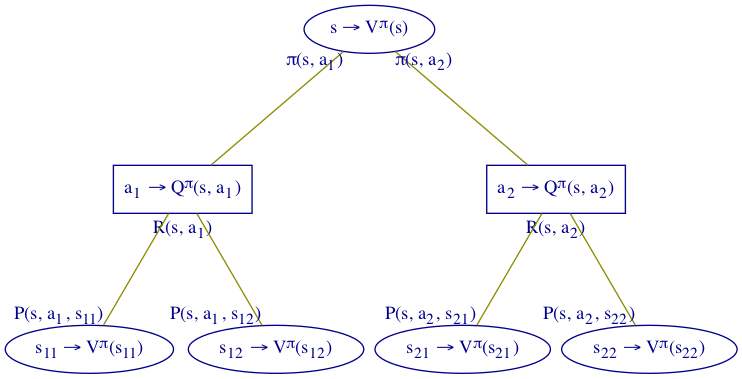
\includegraphics[width=12cm, height=8cm]{mdp_bellman_policy_tree_vv.png}
\end{frame}


\begin{frame}
\frametitle{MDP Action-Value Function Bellman Policy Equation}
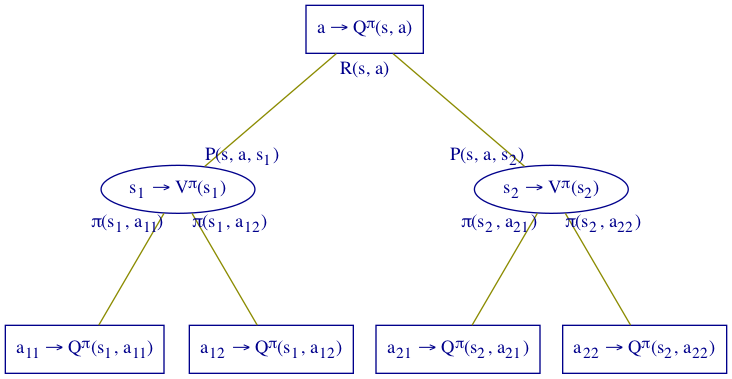
\includegraphics[width=12cm, height=8cm]{mdp_bellman_policy_tree_qq.png}
\end{frame}

\begin{frame}
\frametitle{Optimal Value Functions}
\pause
\begin{itemize}[<+->]
\item {\em Optimal State-Value Function} $V^*: \mathcal{N} \rightarrow \mathbb{R}$ defined as:
$$V^*(s) = \max_{\pi \in \Pi} V^{\pi}(s) \text{ for all } s \in \mathcal{N}$$
where $\Pi$ is the space of all stationary (stochastic) policies
\item {\em For each} $s$, maximize $V^{\pi}(s)$ across choices of $\pi \in \Pi$
\item Does this mean we could have different maximizing $\pi$ for different $s$?
\item We'll answer this question later
\item {\em Optimal Action-Value Function} $Q^*: \mathcal{N} \times \mathcal{A} \rightarrow \mathbb{R}$ defined as:
$$Q^*(s, a) = \max_{\pi \in \Pi} Q^{\pi}(s, a) \text{ for all } s \in \mathcal{N}, a \in \mathcal{A}$$
\end{itemize}
\end{frame}

\begin{frame}
\frametitle{Bellman Optimality Equations}
\pause
\begin{equation}
V^*(s) = \max_{a\in \mathcal{A}} Q^*(s,a)
\label{eq:mdp_bellman_opt_eqn_vq}
\end{equation}
\pause
\begin{equation}
Q^*(s,a) = \mathcal{R}(s,a) + \gamma \cdot \sum_{s' \in \mathcal{N}} \mathcal{P}(s,a,s') \cdot V^*(s')
 \label{eq:mdp_bellman_opt_eqn_qv}
\end{equation}
\pause
These yield the {\em MDP State-Value Function Bellman Optimality Equation}
\begin{equation}
V^*(s) = \max_{a\in \mathcal{A}} \{ \mathcal{R}(s,a) + \gamma \cdot \sum_{s' \in \mathcal{N}} \mathcal{P}(s,a,s') \cdot V^*(s') \}
\label{eq:mdp_bellman_opt_eqn_vv}
\end{equation}
\pause
and the {\em MDP Action-Value Function Bellman Optimality Equation}
\begin{equation}
Q^*(s,a) = \mathcal{R}(s,a) + \gamma \cdot \sum_{s' \in \mathcal{N}} \mathcal{P}(s,a,s') \cdot \max_{a'\in \mathcal{A}} Q^*(s',a')
\label{eq:mdp_bellman_opt_eqn_qq}
\end{equation}
\pause
{\bf MDP Control Problem:} Computing $V^*(\cdot)$ and $Q^*(\cdot)$
\end{frame}

\begin{frame}
\frametitle{MDP State-Value Function Bellman Optimality Equation}
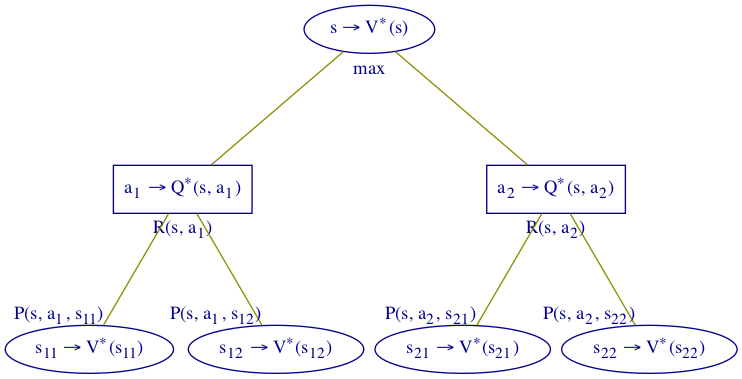
\includegraphics[width=12cm, height=8cm]{mdp_bellman_opt_tree_vv.png}
\end{frame}

\begin{frame}
\frametitle{MDP Action-Value Function Bellman Optimality Equation}
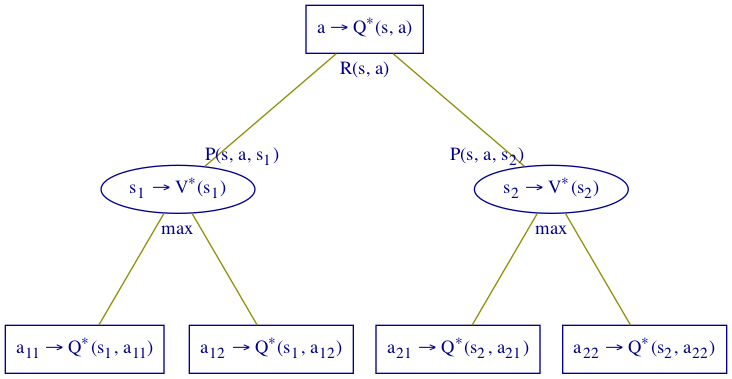
\includegraphics[width=12cm, height=8cm]{mdp_bellman_opt_tree_qq.png}
\end{frame}

\begin{frame}
\frametitle{Optimal Policy}
\pause
\begin{itemize}[<+->]
\item Bellman Optimality Equations don't directly solve {\em Control}
\item Because (unlike Bellman Policy Equations), these are non-linear
\item But these equations form the foundations of DP/RL algos for Control
\item But will solving Control give us the {\em Optimal Policy}?
\item What does {\em Optimal Policy} mean anyway?
\item What if different $\pi$ maximize $V^{\pi}(s)$ for different $s$?
\item So define an {\em Optimal Policy} $\pi^*$ as one that "dominates" all other $\pi$:
$$\pi^* \in \Pi \text{ is an Optimal Policy if } V^{\pi^*}(s) \geq V^{\pi}(s) \text{ for all } \pi \text{ {\em and} for all } s$$
\item Is there an Optimal Policy $\pi^*$ such that $V^*(s) = V^{\pi^*}(s)$ for all $s$?
\end{itemize}
\end{frame}

\begin{frame}
\frametitle{Optimal Policy achieves Optimal Value Function}
\begin{theorem}
For any (discrete-time, countable-spaces, stationary) MDP:
\pause
\begin{itemize}[<+->]
\item There exists an Optimal Policy $\pi^* \in \Pi$, i.e., there exists a Policy $\pi^* \in \Pi$ such that $V^{\pi^*}(s) \geq V^{\pi}(s) \text{ for all policies  } \pi \in \Pi \mbox{ and for all states } s \in \mathcal{N}$
\item All Optimal Policies achieve the Optimal Value Function, i.e. $V^{\pi^*}(s) = V^*(s)$ for all $s \in \mathcal{N}$, for all Optimal Policies $\pi^*$
\item All Optimal Policies achieve the Optimal Action-Value Function, i.e. $Q^{\pi^*}(s,a) = Q^*(s,a)$ for all $s \in \mathcal{N}$, for all $a \in \mathcal{A}$, for all Optimal Policies $\pi^*$
\end{itemize}
\label{th:optimal-policy-achieves-optimal-value-function}
\end{theorem}
\end{frame}

\begin{frame}
\frametitle{Proof Outline}
\pause
\begin{itemize}[<+->]
\item For any Optimal Policies $\pi_1^*$ and $\pi_2^*$, $V^{\pi_1^*}(s) = V^{\pi_2^*}(s)$ for all $s \in \mathcal{N}$
\item Construct a candidate Optimal (Deterministic) Policy $\pi_D^* : \mathcal{N} \rightarrow \mathcal{A}$:
 $$\pi_D^*(s) = \argmax_{a \in \mathcal{A}} Q^*(s,a) \text{ for all } s \in \mathcal{N}$$
 \item $\pi_D^*$ achieves the Optimal Value Functions $V^*$ and $Q^*$:
 $$V^*(s) = Q^*(s,\pi_D^*(s)) \text{ for all } s \in \mathcal{N}$$
 $$V^{\pi_D^*}(s) = V^*(s) \text{ for all } s \in \mathcal{N}$$
$$Q^{\pi_D^*}(s,a) = Q^*(s,a) \text{ for all } s \in \mathcal{N}, \text{ for all } a \in \mathcal{A}$$
\item $\pi_D^*$ is an Optimal Policy:
$$V^{\pi_D^*}(s) \geq V^{\pi}(s) \text{ for all policies  } \pi \in \Pi \text{ and for all states } s \in \mathcal{N}$$
\end{itemize}
\end{frame}

\begin{frame}
\frametitle{State Space Size and Transitions Complexity}
\pause
\begin{itemize}[<+->]
\item Tabular Algorithms for State Spaces that are not too large
\item In real-world, state spaces are very large/infinite/continuous
\item {\em Curse of Dimensionality}: Size Explosion as a function of dimensions
\item {\em Curse of Modeling}: Transition Probabilities hard to model/estimate
\item Dimension-Reduction techniques, Unsupervised ML methods
\item Function Approximation of the Value Function (in ADP and RL)
\item Sampling, Sampling, Sampling ... (in ADP and RL)
\end{itemize}
\end{frame}

\begin{frame}
\frametitle{Action Space Sizes}
\pause
\begin{itemize}[<+->]
\item Large Action Spaces: Hard to represent, estimate and evaluate:
\begin{itemize}
\item Policy $\pi$
\item Action-Value Function for a policy $Q^{\pi}$
\item Optimal Action-Value Function $Q^*$
\end{itemize}
\item Large Actions Space makes it hard to calculate $\argmax_a Q(s,a)$
\item Optimization over Action Space for each non-terminal state
\item Policy Gradient a technique to deal with large action spaces
\end{itemize}
\end{frame}

\begin{frame}
\frametitle{Time-Steps Variants and Continuity}
\pause
\begin{itemize}[<+->]
\item Time-Steps: terminating ({\em episodic}) or non-terminating ({\em continuing})
\item Discounted or Undiscounted MDPs, Average-Reward MDPs
\item Continuous-time MDPs: Stochastic Processes and Stochastic Calculus
\item When States/Actions/Time all continuous, Hamilton-Jacobi-Bellman
\end{itemize}
\end{frame}

\begin{frame}
\frametitle{Partially-Observable Markov Decision Process (POMDP)}
\pause
\begin{itemize}[<+->]
\item Two different notions of {\em State}:
\begin{itemize}
\item Internal representation of the environment at each time step $t$ ($S_t^{(e)}$)
\item The agent's state at each time step $t$ (let's call it $S_t^{(a)}$)
\end{itemize}
\item We assumed $S_t^{(e)} = S_t^{(a)} (= S_t)$ and that $S_t$ is {\em fully observable}
\item A more general framework assumes agent sees {\em Observations} $O_t$
\item Agent cannot see (or infer) $S_t^{(e)}$ from history of observations
\item This more general framework is called {\em POMDP}
\item POMDP is specified with {\em Observation Space} $\mathcal{O}$ and observation probability function 
$\mathcal{Z}: \mathcal{S} \times \mathcal{A} \times \mathcal{O} \rightarrow [0, 1]$
defined as:
$$\mathcal{Z}(s', a, o) = \mathbb{P}[O_{t+1} = o | (S_{t+1} = s', A_t = a)]$$
\item Along with the usual transition probabilities specification $\mathcal{P}_R$
\item MDP is a special case of POMDP with $O_t = S_t^{(e)} = S_t^{(a)} = S_t$
\end{itemize}
\end{frame}

\begin{frame}
\frametitle{POMDP Framework}
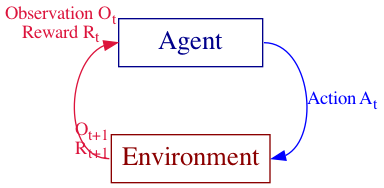
\includegraphics[width=12cm, height=8cm]{pomdp.png}
\end{frame}

\begin{frame}
\frametitle{Belief States, Tractability and Modeling}
\pause
\begin{itemize}[<+->]
\item Agent doesn't have knowledge of $S_t$, only of $O_t$
\item So Agent has to ``guess'' $S_t$ by maintaining {\em Belief States}
$$b(h)_t = (\mathbb{P}[S_t=s_1 | H_t = h], \mathbb{P}[S_t = s_2 | H_t = h], \ldots )$$
where history $H_t$ is all data known to agent by time $t$:
$$H_t := (O_0, R_0, A_0, O_1, R_1, A_1, \ldots, O_t, R_t)$$
\item $H_t$ satisfies Markov Property $\Rightarrow  b(h)_t$ satisfies Markov Property
\item POMDP yields (huge) MDP whose states are POMDP's belief states
\item Real-world: Model as accurate POMDP or approx as tractable MDP?
\end{itemize}
\end{frame}

\begin{frame}
\frametitle{Key Takeaways from this Chapter}
\pause
\begin{itemize}[<+->]
\item MDP Bellman Policy Equations
\item MDP Bellman Optimality Equations
\item Existence of an Optimal Policy, and of each Optimal Policy achieving the Optimal Value Function
\end{itemize}
\end{frame}


\end{document}